% Conceptual DP state and transition lattice.
% Stages t on the x axis, discrete SoC levels on the y axis. From one state a
% few actions lead to nearby SoC levels: charge moves up, discharge moves down,
% idle stays level. Only a small grid is drawn for clarity.
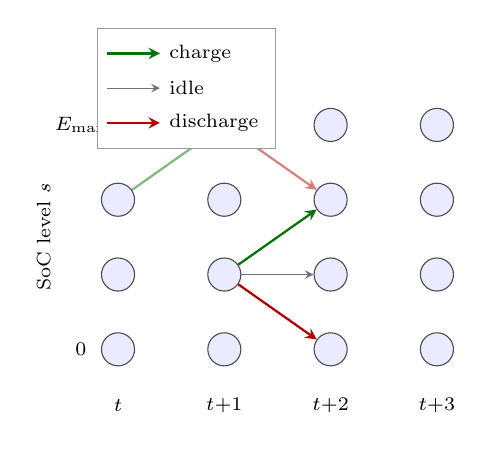
\begin{tikzpicture}[
    x=1.35cm, y=0.95cm,
    node distance=0pt,
    state/.style={circle, draw=black!70, fill=blue!8, minimum size=4.2mm,
                  inner sep=0pt, font=\scriptsize},
    chg/.style={->, >=stealth, green!45!black, thick},
    dis/.style={->, >=stealth, red!70!black, thick},
    idle/.style={->, >=stealth, black!55},
]
% Grid of states: 4 stages, 4 SoC levels.
\foreach \t in {0,1,2,3} {
  \foreach \s in {0,1,2,3} {
    \node[state] (n\t\s) at (\t,\s) {};
  }
}
% Stage labels.
\foreach \t/\lab in {0/{$t$},1/{$t{+}1$},2/{$t{+}2$},3/{$t{+}3$}} {
  \node[font=\scriptsize] at (\t,-0.75) {\lab};
}
% SoC axis label.
\node[rotate=90, font=\scriptsize] at (-0.7,1.5) {SoC level $s$};
\node[font=\scriptsize] at (-0.35,0) {$0$};
\node[font=\scriptsize] at (-0.35,3) {$E_{\max}$};

% Sample transitions out of state (n11): charge up, idle, discharge down.
\draw[chg]  (n11) -- (n22);
\draw[idle] (n11) -- (n21);
\draw[dis]  (n11) -- (n20);
% A couple more to suggest the full fan-out.
\draw[chg, opacity=0.5]  (n02) -- (n13);
\draw[dis, opacity=0.5]  (n13) -- (n22);

% Legend.
\matrix[draw=black!40, fill=white, inner sep=3pt, row sep=1pt,
        anchor=north west, font=\scriptsize] at (-0.2,4.3) {
  \draw[chg] (0,0) -- (0.5,0); & \node[anchor=west] {charge}; \\
  \draw[idle] (0,0) -- (0.5,0); & \node[anchor=west] {idle}; \\
  \draw[dis] (0,0) -- (0.5,0); & \node[anchor=west] {discharge}; \\
};
\end{tikzpicture}
